
\documentclass[a4paper, 11pt]{article}

\usepackage{verbatim}
\usepackage{pdfpages}
\usepackage[T1]{fontenc}
\usepackage{titling}
\usepackage{amsmath}
\usepackage{amsfonts}
\usepackage{graphicx}
\usepackage{mathtools}
\usepackage[includeheadfoot,margin=23mm]{geometry}
\usepackage{multirow}
\usepackage{xfrac}
\usepackage{epstopdf}
\usepackage{float}
\makeatletter
\newcommand{\sectionauthor}[1]{}
\makeatother
\usepackage[bottom]{footmisc}
\usepackage{helvet}
\renewcommand{\familydefault}{\sfdefault}

\usepackage{chngcntr}
\counterwithin{figure}{section}

\usepackage{caption}
\usepackage{subcaption}

\usepackage{gensymb}

\usepackage{setspace}
\doublespacing

\usepackage{fancyhdr}
\pagestyle{fancy}
\cfoot{\fancyplain{}{\thepage}}

\usepackage{fancyhdr}
\pagestyle{fancy}
\fancypagestyle{wojciech}{
	\fancyhead{} % clear all header fields
	\lhead{\leftmark }
	\rhead{Wojciech Dziwulski}
	\cfoot{\thepage}
}


\usepackage{titlesec}
\setcounter{secnumdepth}{4}
\titleformat{\paragraph}
{\normalfont\normalsize\bfseries}{\theparagraph}{1em}{}
\titlespacing*{\paragraph}
{0pt}{3.25ex plus 1ex minus .2ex}{1.5ex plus .2ex}
\usepackage{gensymb}



\renewcommand{\headrulewidth}{0.5pt}

\numberwithin{equation}{section}
\usepackage[numbered, framed]{matlab-prettifier}

\lstset{
	style              = Matlab-editor,
	escapechar         = ",
	mlshowsectionrules = true,
	tabsize            = 2,
}

\graphicspath{{Images/}}

\setlength{\droptitle}{-8em}

\title{Distributed Neural Network Training \\ \large Final Year Project}

\author{\textbf{Wojciech Dziwulski}}

\date{}

\begin{document}
	
	\clearpage
	\maketitle
	\thispagestyle{empty}
	\begin{abstract}
		The project investigates the ways of breaking down deep neural network processing between several computational units. It first introduces some background information about machine intelligence and deep learning. Some existing approaches to the problem are summarized based on a relevant literature review. A novel strategy for distributing the computation is set out and various deep learning frameworks are evaluated to lead to a conclusive choice. The advantages and disadvantages of the framework are summarized, in addition to some baseline results of the proposed framework's implementation.
		
	\end{abstract}
	
	
	\newpage
	\pagenumbering{roman}
	\tableofcontents 
	
	
	\newpage
	\pagenumbering{arabic}
	
	
	\clearpage
	
	
	\newpage
	
	\clearpage
	
	\pagestyle{wojciech}
	
	\section{Introduction}
	
	Understanding data was the cornerstone of humanity's development, its greatest feat and challenge. It is undoubtedly the reason why we become rational beings, even though we come to this world blissfully helpless. Due to the rapid technological revolution of the past few decades we now produce more data than was previously imaginable, and hence develop novel techniques for making sense of it. The data we produce, however, is as diverse as it is abundant, with different data sets requiring very different analysis and treatment. Classifying emails as spam is clearly a task whole lot different than image recognition, which is in turn dissimilar to natural language processing.
	
	For simplicity, let's look at the spam classification example. We can imagine the data as points occupying a multi-dimensional space. The point coordinates describe its features - in our case the occurence of fraudulent clauses, grammar correctness, legitimacy of the email address and many more. Based on those features, we can try to draw a classification boundary - for example a hyperplane dividing the bad from the good, \textbf{to the extent that our algorithm can work it out}. Not every algorithm will come up with the same boundary, though, and only some will come up with a valid one. This depends on the characteristics of the dataset.
	
	The most rudimentary way of describing the interdependencies between variables in the set is their linearity. If we can describe the classification boundary by a function linear in its coefficients, then we call the dataset linear. Most of algorithms can deal with this sort of datasets quite well. In fact, if we extend our discussion to regression, the learning problem has already been approached in the 19th century. This is because even fitting a best-fit line to a set of points on a 2D plane lets us detect trends in the data. Problem arises when the dataset is not linearly separable - if there is a more subtle relationship between the data features. Sadly for linear regression, but excitingly for the development of science, most of the "natural" datasets we study are not linear. \textbf{Machine learning} is the field concerned with developing techniques robust to the dataset charasteristics and bringing the technology closer to the sophistication with which the humans understand the world.
	
	Interestingly the problems that we, humans, find awfully easy, such as informed vision, turn out to be tremendously hard for the computers to perform. Our brains are amazingly complicated machines, with the computational power available at a very low energetic cost. Millions of years of evolution equipped us with skills that are impossible to replicate with the current technology, which certainly doesn't mean we shouldn't try, though! The research on human visual cortex (Kruger et al., 2013 \cite{kruger2013deep}), for example, gave us significant insight into the generalised machine vision problems, and stimulated the development of a field known as deep learning.
	
	Current technology allows us to achieve tremendous image classification results, but novel methods need to be developed in order to tackle the new challenges. It turns out that the complexity of the functions a neural network can learn increases with the increasing depth of the net itself. To construct a truly deep network, though, we need more space for computation, which we can achieve by distributing the computation among many distinct servers. This approach will ideally be indistinguishable to the outside world from a training a single network and should lead to similar, if not better, classification results. Before we delve into the technical details of the distributed training itself, though, let's revisit some basic machine learning concepts first in order to establish a solid grounding for the later considerations.
	
	\section{Background - machine intelligence}
	
	\subsection{Neural networks}
	
	\cite{ng2015coursera} It was noted at the end of the previous section that linear regression's most obvious drawback is the inability to cope with non-linear datasets. With the use of non-linear transformation of variables we could, in theory, produce features that are linearly separable, however it is often impossible to guess the correct transformation. Besides, expanding the feature set to include the non-linearities (e.g. quadratic cross feature products) would grow the storage space unreasonably. Both random forests and artificial neural networks are in theory able to address that problem. Their inherently non-linear architectures help conforming to more diverse and complex classification challenges. \\
	
	As the name suggests, the artificial neural networks are loosely based on the human brain's intricate internal architecture. Their most basic building block is a logistic unit, which works similarly to a logistic regression classifier.
	
	\begin{figure}[!h]
		\centering
		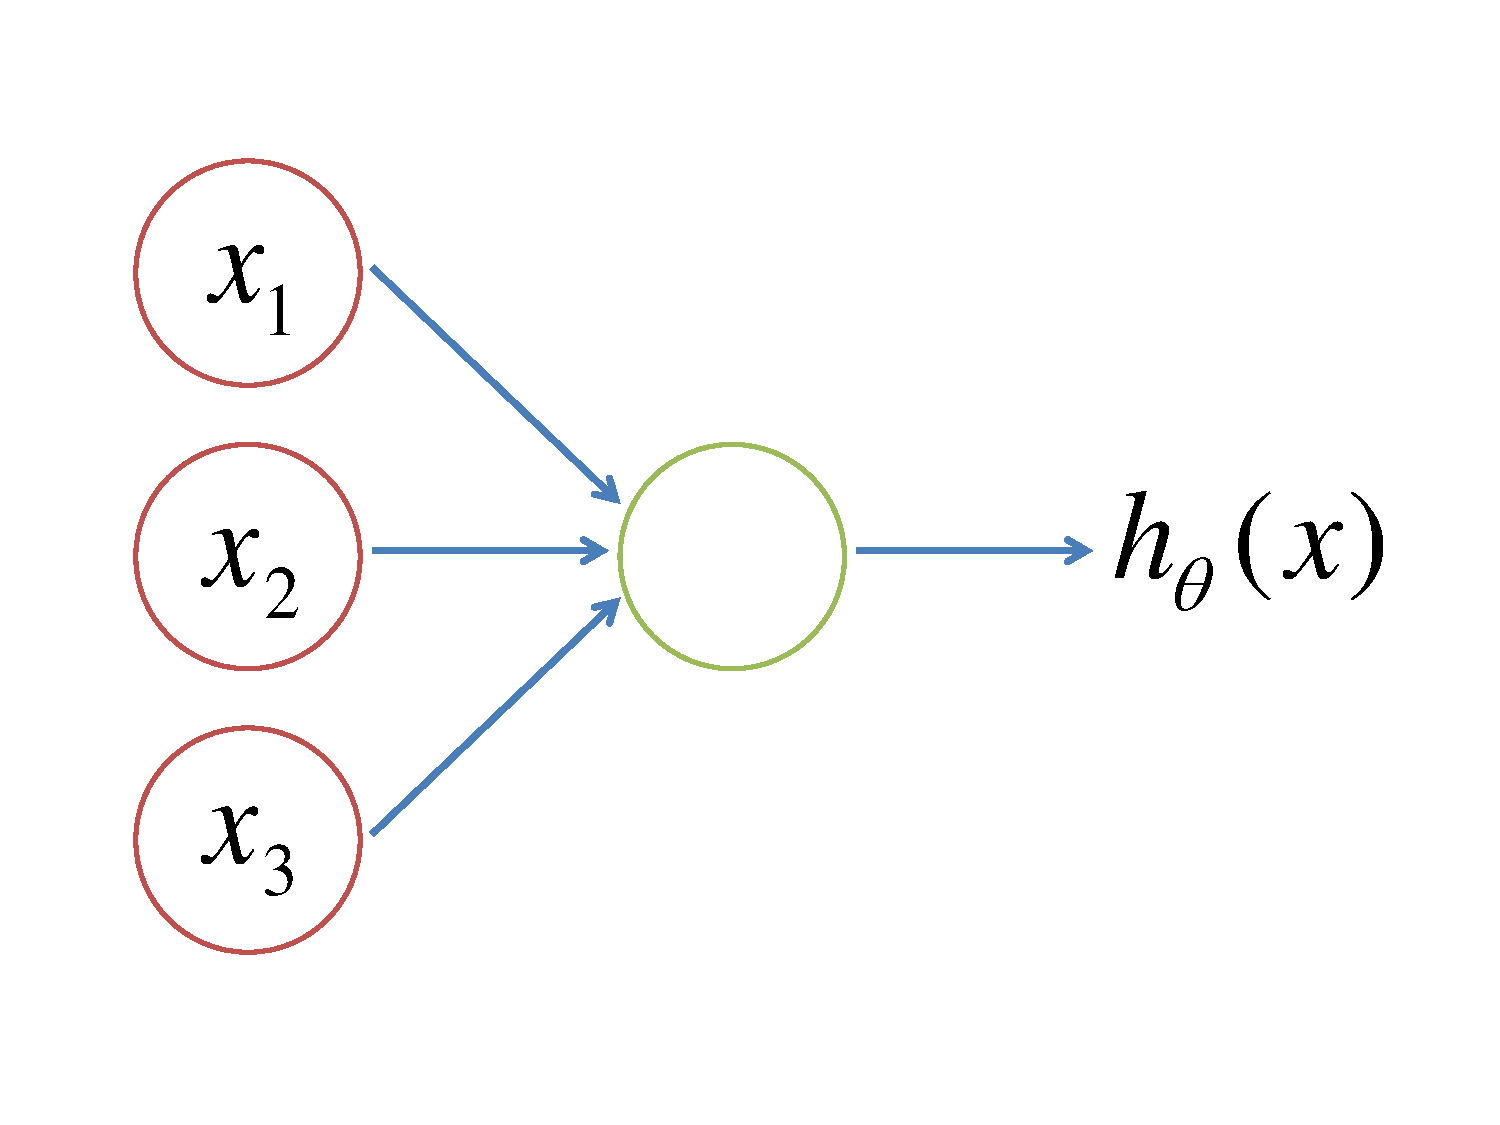
\includegraphics[page=1,width=0.40\textwidth]{logistic_unit.pdf}
		\caption{\label{fig:logistic_unit}{A logistic unit}}
	\end{figure}
	
	The logistic unit takes in input features $x_1, x_2, ..., x_n$ and makes an output decision using a logistic sigmoid function, i.e. (as before):
	
	\begin{equation}
	h_\theta (x) = \frac{1}{1+e^{-\theta ^ T x}}
	\end{equation}
	where $\theta$ are the feature weights.\\
	
	Naturally, many more of those logistic units are combined within a layer of a neural net and many more layers are combined to form a neural network (see fig. \ref{fig:neural_net}). It comprises of one input and one output layer, in addition to several (in case of the aforementioned figure just one) hidden layers. For a three layer network with three nodes in each layer, output is calculated according to:
	
	\begin{align}
	a_1^{(2)} &= \sigma (\Theta_{10}^{(1)} x_0 + \Theta_{11}^{(1)} x_1  + \Theta_{12}^{(1)} x_2  + \Theta_{13}^{(1)} x_3) \\
	a_2^{(2)} &= \sigma (\Theta_{20}^{(1)} x_0 + \Theta_{21}^{(1)} x_1  + \Theta_{22}^{(1)} x_2  + \Theta_{23}^{(1)} x_3) \\
	a_3^{(2)} &= \sigma (\Theta_{30}^{(1)} x_0 + \Theta_{31}^{(1)} x_1  + \Theta_{32}^{(1)} x_2  + \Theta_{33}^{(1)} x_3) \\
	\Rightarrow h_{\Theta} (x) &= \sigma (\Theta_{10}^{(2)} \boldsymbol{a_0} + \Theta_{11}^{(2)} \boldsymbol{a_1}  + \Theta_{12}^{(2)} \boldsymbol{a_2}  + \Theta_{13}^{(2)} \boldsymbol{a_3})
	\end{align}
	where the superscript denotes the layer number and the subscripts denote the output and input node index respectively. More compactly:
	\begin{align}
	a^{(2)} = \sigma(\Theta^{(1)} x^{(1)}) \\
	h_{\Theta}(x) = \sigma(\Theta^{(2)} a^{(2)})
	\end{align}
	
	\begin{figure}[!h]
		\centering
		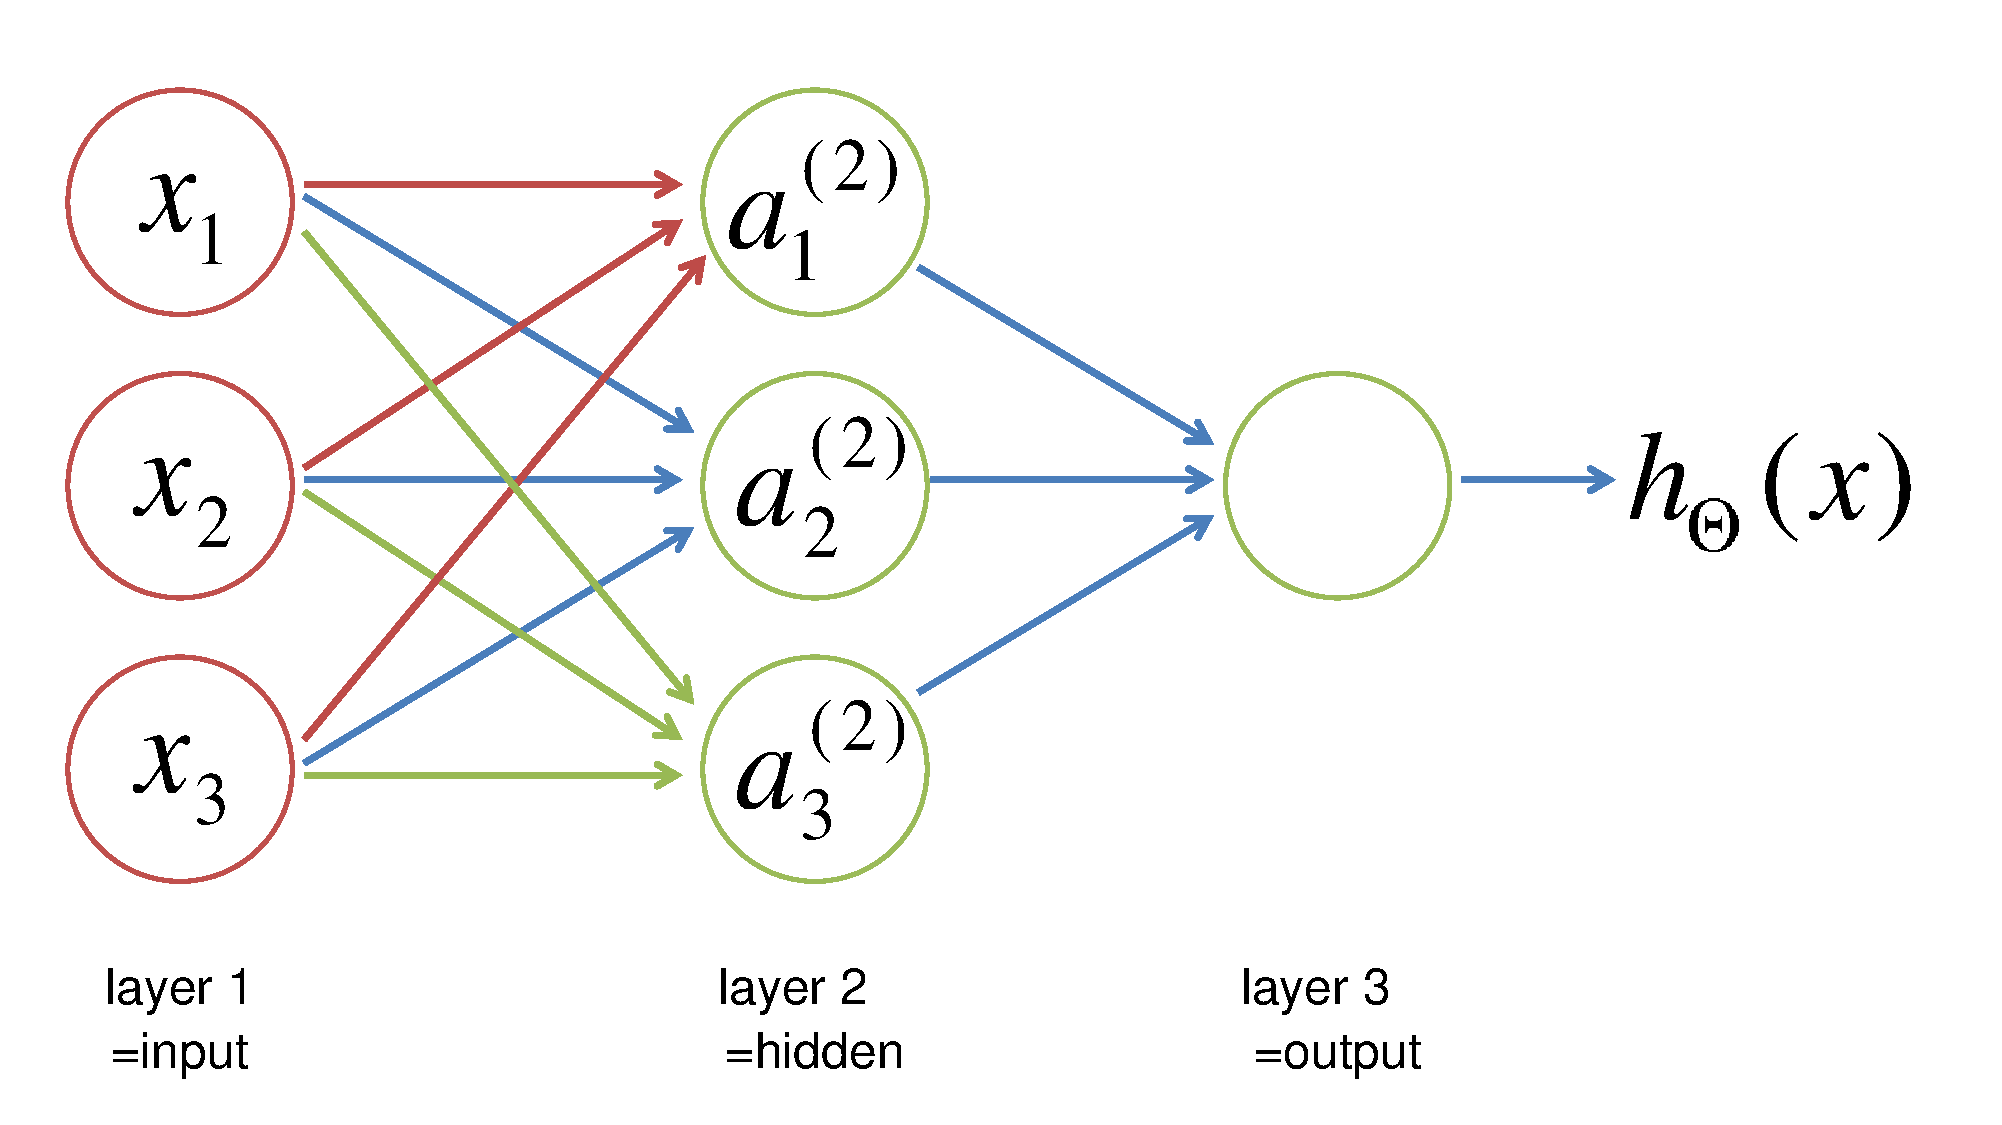
\includegraphics[page=1,width=0.60\textwidth]{neural_net.pdf}
		\caption{\label{fig:neural_net}{A simple neural net}}
	\end{figure}
	
	The computation above is called forward propagation, because it sequentially calculates the activation value $a$ for particular layers of logistic units using the previous ones. Now the most important feature of the neural nets is that the features within the layers (e.g. $a_1^{(2)}, a_2^{(2)}, a_3^{(2)}$) are "learnt" automatically, by appropriately tweaking the $\Theta$ vector using an algorithm called the back propagation. We adjust the weights so as to minimize the overall loss function of the network.
	
	In case of the neural networks, the loss function is defined as:
	\begin{equation}
	J(\Theta) = - \frac{1}{m} \Bigg[\sum_{i=1}^{m} \sum_{k=1}^{K} y_k^{(i)}log(h_\Theta(x^{(i)}))_k + (1-y_k^{(i)}) log(1-(h_\Theta(x^{(i)}))_k) \Bigg] + \frac{\lambda}{2m} \sum_{l=1}^{L-1} \sum_{i=1}^{s_l} \sum_{j=1}^{s_{l+1}} (\Theta _ {ji} ^{(l)})^2
	\end{equation}
	where $l$ is the network layer number, $L$ is the total number of layers, $s_l$ is the number of layers in layer $l$ and $K$ is the number of output units. The first term tries to minimize the difference between the classification computed by the network and the true label. The second term ($\frac{\lambda}{2m} \ldots$) is a regularization term included to prevent the values of the weights from becoming very big.
	In order to minimize the cost, we also need to know how to compute the gradient with respect to individual connection weights within the nets i.e.:
	\begin{equation}
	\frac{\partial}{\partial \Theta_{ij}^{(l)}} J(\Theta))
	\end{equation}
	
	That is where the back propagation comes into play. To illustrate its operation, we can assume being given one training example $(x, y)$ for which, using a randomly initialized neural net, we run the first forward propagation sweep to obtain the initial prediction:
	\begin{align}
	a^{(1)} &= x \\
	a^{(2)} &= \sigma(\Theta^{(1)} a^{(1)}) \\
	&\ldots \\
	a^{(L)} &= h_{\Theta}(x)= \sigma(\Theta^{(L-1)} a^{(L-1)})
	\end{align}
	
	Now, starting from the output layer of the net, we can compute the "error", whose value will help us obtain the gradient:
	\begin{align}
	\delta^{(L)} &= a^{(L)} - y \quad \textrm{for the last layer} \\
	\delta^{(L-1)} &= (\Theta ^ {(L-1)})^T \delta^{(L)} \cdot \sigma'(\Theta^{(L-2)} a^{(L-2)}) \\
	&\ldots \\
	\delta^{(2)} &= (\Theta ^ {(2)})^T \delta^{(3)} \cdot \sigma'(\Theta^{(1)} a^{(1)})
	\end{align}
	where $\sigma'$ is the derivative of the logistic sigmoid, which is easily computed as:
	\begin{align}
	\sigma'(\Theta^{(n)} a^{(n)}) = a^{(n+1)} \cdot (1-a^{(n+1)})
	\end{align}
	Now, incidentally, it can be shown that:
	\begin{equation}
	\frac{\partial}{\partial \Theta_{ij}^{(l)}} J(\Theta)) = a_j^{(l)} \delta_i^{(l+1)}
	\end{equation}
	
	Given that we know how to calculate the gradient, we can now try to minimize the cost function using gradient descent. As the number of iterations of back propagation increases, the forward propagation sweeps through the net should yield results closer and closer to the ground truth.
	
	\subsection{Gradient descent}
	The loss minimization problems often involve gradient methods, such as gradient descent. To see why that is, we note that wherever we find outselves on the graph of a function, we can find the local minimum neighbouring our current location by following the function's negative gradient, i.e. the direction where the function is monotonously decreasing. Once we hit a point where we can't minimize any further, we are at the minimum. Gradient descent does precisely that - it first calculates the derivative of the function and follows the direction that will result in the loss minimization, which can be clearly seen in the figure \ref{fig:graddesc} below.
	
	\begin{figure}[!h]
		\centering
		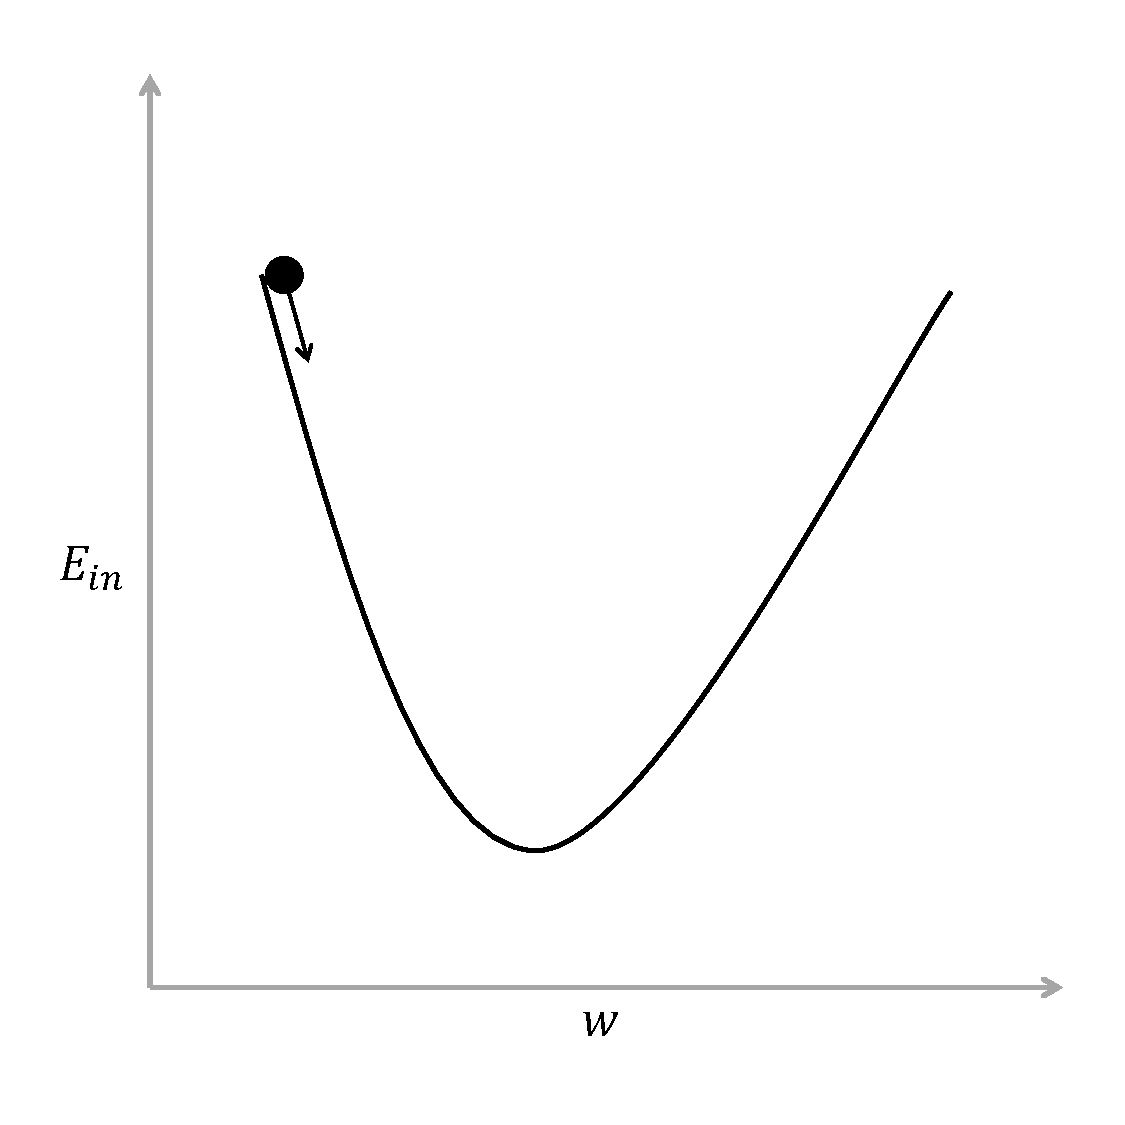
\includegraphics[page=1,width=0.40\textwidth]{graddesc.pdf}
		\caption{\label{fig:graddesc}{We follow the function in the negative gradient direction.}}
	\end{figure}
	
	We can write down an equation summarizing the weight update throughout the network in terms of the gradient of the in-sample error with respect to the weight vector.
	\begin{align}
	\Delta w &= - \eta \nabla E_{in}(w) \\
	\textrm{where:} \quad E_{in} &= \frac{1}{N} \sum_{n = 1}^{N} e(h(x_n), y_n)
	\end{align}
	
	If we calculate the gradient of the loss function based on all of the points as above, we use a variant of the gradient descent algorithm called "batch" GD. It turns out, though, that such a method is extremely computationally engaging, particularly noting how large the datasets can be nowadays!
	
	Instead, we can use a technique called "stochastic" gradient descent. Its correctness is guaranteed by the assumption that if we use a random sample of the whole training set many times, the computed gradients will average out to give a globally correct answer. In an extreme case, we only use one data point to calculate the gradient, however for stability purposes we can use image batches of up to a few hundred images. This is neatly summarized by the modified version of the equation above:
	\begin{align}
	\Delta w &= - \eta \nabla E_{sample}(w) \\
	\textrm{where:} \quad E_{sample} &= \frac{1}{N_{sample}} \sum_{n = 1}^{N_{sample}} e(h(x_n), y_n)
	\end{align}
	
	\subsection{Deep learning}
	
	As mentioned before (Kruger at al., 2014 \cite{kruger2013deep}), human visual cortex and deep learning have, or at least are meant to have, a lot in common. Based on the research on the visual cortex, we can characterise the human vision and perception by its structural composition. It is apparent, that the neural structure is hierarchical, in that the visual impulses pass through consecutive stages of processing before identification. The lower "layers" of the cortex distinguish the simple image features over specialised regions and then pass on the information to the higher areas which are able to identify increasingly higher level context of the image.
	
	The technical complexity of the process is supported by the computational efficiency of the structure. The cortical areas share feature recognition information to enable straightforward storage and processing. Because of the hierarchical structure of the visual cortex and the large number of processing layers that are passed before final classification, such structures are called "deep" and are able to achieve tremendous efficiency. It was proven before that for an arbitrary function f(x) compactly represented by a depth \textbf{l} network, we might require an \textbf{exponentially large number} of nodes in a depth \textbf{l-1} network. This certainly sets a good example for engineering artificials structures used for similar purposes.
	
	The reason why we speak about \textbf{convolutional} nets \cite{stanford2016convnets} is that our artificial neurons are in this case convolutional filters that we apply to the outputs of consecutive neural layers. They are the little windows that we dot product with consecutive areas of the input in order to get an "activation map". Each filter generates an activation map of its own, so combined together they assemble a 3d volume of neuron activations. This first step of the computation is, not surprisingly, called the \textbf{convolutional layer}.
	
	What comes next is the ReLU layer of the \textbf{rectified linear unit}, which plays the role of an activation function preventing fading gradients. 
	The \textbf{pooling layer} performs a downsampling operation on the thresholded set, in order to reduce the order of computation.
	Lastly, as in traditional neural nets, there is  a \textbf{fully-connected layer} which constitutes the last step of classification, whose output corresponds to the identified labels.
	
	Since the depth of the convolutional filter is always equal to the depth of its input, the resulting activation map has unit depth (see fig. \ref{fig:conv_net}). To avoid the curse of dimensionality, or explosion of the parameter space size, we assume that the neurons within one activation map share the same weights and bias i.e. if a filter is useful in one area of the image, it will also be useful in the other. Similarly to traditional neural nets, we then use the back-propagation algorithm in order to adjust the neural weights and bias and eventually train the classifier.
	
	\begin{figure}[!h]
		\centering
		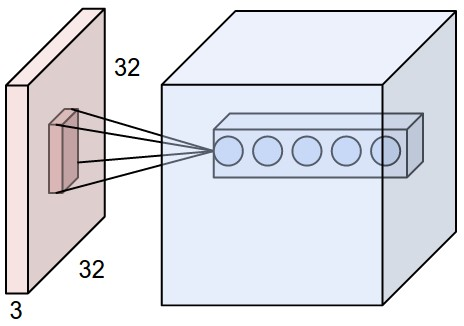
\includegraphics[page=1,width=0.40\textwidth]{depthcol.jpeg}
		\caption{\label{fig:conv_net}{The input volume in red is transformed into a set of 5 activation layers using 5 convolutional filters.}}
	\end{figure} 
	
	\section{Scaling and parallelisation}
	
	It has been proven before (Ciresan et al., 2010 \cite{ciresan2010deep}) that the accuracy of the neural system classification algorithm increases tremendously if large datasets are available. This is consistent with our intuition - the more training examples and the broader the example space, the better we can learn how to replicate the results and correctly classify new data. Even though scaling the datasets is a widely accepted way of improving the classification accuracy, it comes at a significant cost - the time required to train the networks does not expand linearly with the amount of data fed. This poses a significant issue, as the current technology is not capable of training the nets of the desired size. At least not in a sequential manner.
	
	Parallel computation is a technique that greatly speeds up the training by breaking down the outstanding training jobs between different cores of a processor or, ideally, different machines. One advancement in the area came with the realisation that a device perfectly suited for parallel computation is the GPU - Graphical Processing Unit. Whereas the CPU is suited perfectly for sequential tasks, the GPU comes second-to-none when there is a lot of smaller tasks to be handled at the same time. It consists of hundreds of small cores which, although originally designed to render graphics, can be succesfully adapted for the parallelisation of deep learning. Interestingly, the hardware vendors responded extensively to the needs of the scientific (and commercial) machine learning community by providing extensive frameworks for GPU programming (e.g. NVIDIA CUDA).
	
	Even though revolutionary, GPUs can be proved to be insufficient for large neural networking training. As mentioned before, the prediction accuracy scales with the model size, and the amount of data we can fit on a single machine with a couple of GPUs is clearly limited. This explains the need for even grater parallelisation - not only between various cores of the GPU itself, but also between various servers. 
	
	\section{Breaking it down}
	\label{breakingitdown}
	
	Efficient parallelisation between servers turns out to be an extremely complicated task. Considerations regarding net partitioning span several areas, for example:
	\begin{enumerate}
		\item Parallelisation within the individual machines
		\item Partitioning architecture
		\item Storage of net parameter weights and activations
		\item Communication of the newly computed values
		\item Updating conflicting results
		\item Optimization algorithms
	\end{enumerate}
	
	There has been several academic attempts at the problem, most notably: "Large Scale Distributed Deep Networks" (Dean et al., 2012 \cite{dean2012large}) and "Project Adam: Building an Efficient and Scalable Deep Learning Training System" (Chilimbi et al., 2014 \cite{chilimbi2014project}). Both of these are described below with respect to their solutions to the enumerated problems.
	
	\subsection{Large Scale Distributed Deep Networks}
	
	The paper focuses on two advencements developed by the authors: a software framework called \textbf{DistBelief} as well as two algorithms: \textbf{Downpour SGD} and \textbf{Sandblaster L-BFGS}. DistBelief can be considered a solution to problems 1-5 listed in section \ref{breakingitdown}, whereas the two algorithms are optimization procedures tailored for the highly distributed network training.
	
	\begin{figure}[H]
		\centering
		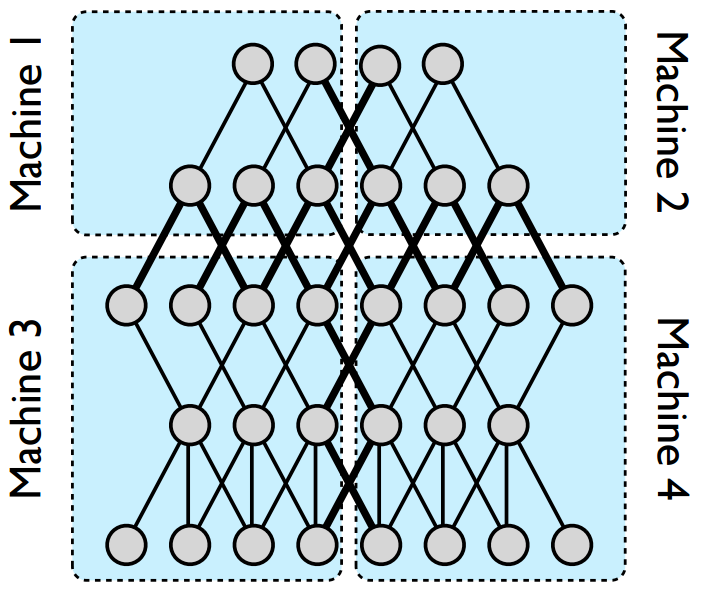
\includegraphics[width=0.40\textwidth]{distbelief.png}
		\caption{\label{fig:distbelief}Example model architecture in DistBelief \cite{dean2012large}}
	\end{figure}
	
	The DistBelief framework is a comprehensive tool that lets the user define the net architecture (fig. \ref{fig:distbelief}) and computation in the chosen nodes. There is no extra user intervention required - the framework takes care of the intra-machine parallelism as well as communication between the machines. Interestingly, splitting the net across several machines does not always yield the most optimal results - it might easily be the case that the communication costs prevail and the overall process is slowed down due to inter-machine parallelism. In addition to communication inefficiencies, different machines will also complete their workload in different time, hence wasting the computational resources and leading to slowdowns.
	
	One of the most common optimization algorithms is Stochastic Gradient Descent. It is extremely versatile and has a myriad of applications, however due to its inherently sequential character it is hard to simply apply it to a highly parallelised problem. The paper hence proposed an asynchronous variant of SGD - Downpour. The training data is broken down and trained on separate copies of the model which run independently of each other. The algorithm is highly randomised, and there is little guarantee the asynchronous parameter updates will be in-order or will not result in data loss. As the authors point out, though, this relaxation brings about effective results. Another improvement is using separate learning rates for various parameters (Adagrad).
	
	An alternative optimization procedure presented in the paper is Sandblaster L-BFGS. As opposed to typical BFGS, the model replicas are assigned much smaller data portions. This mitigates the impact of slow machines, which just process a smaller portion of data in the alloted time, as compared to the better performing units.		 
	
	\subsection{Project Adam}
	
	Project Adam is a framework somewhat resembling the one described above. It supports the highly parallelised computation, however, as a newer technology, it also offers a couple of improvements.
	
	Adam architecture devotes several machines exclusively for \textbf{data serving}, including the necessary data processing beforehand. In the visual tasks, in order to proliferate the data sets images undergo multiple transformations such as reflections and rotations. Decoupling data serving compute-load from the actual network training specialises the machines in the given tasks and hence speeds up the overall process.
	
	Due to the highly parallelised nature of the framework, there are several characteristics of the architecture that are worth mentioning. First of all, the training on each of the machines is multi-threaded. The threads share the network parameters and, what is more imporant, update them without using locks. This of course implies that the updates are not guaranteed to be based on the latest version of the model, but the training was proven robust enough to converge even in the presence of the noise. As mentioned earlier, the uneven processing times between the machines is a significant bottleneck of the process. Adam architecture tries to mitigate this by finishing an epoch processing after only 75\% of the model replicas have terminated computation.
	
	The shared parameter server is another crucial part of the platform. Due to the high computational demand, it breaks down the model parameters into 1MB shards hashed into storage buckets. This is in contrast to the conventional key-value store.
	
	\subsection{Contrast and conclusions}
	
	The two architectures described in the sections before are very distinct, although they share common problems and hence offer some similar solutions. They have both achieved impressive classification results in the 21k category ImageNet classification task - over 15\% accuracy for DistBelief and stunning 29.8\% for the Adam architecture.
	
	The most important takeaways from the papers are:
	\begin{itemize}
		\item There are two distinct ways of dealing with the slow machine bottleneck. One is to break down the computation into much smaller loads and process them gradually as the machines become available (DistBelief). The other is to finish computation after a fraction of the model replicas have finished processing (Adam). Both speed up the training, although the latter clearly introduces some information loss.
	\end{itemize}
	
	\section{ADMM}
	\label{ADMM}
	
	Alternating Direction Method of Multipliers is an algorithm for solving constrained optimisation problems. It is based on the augmented Lagrangian method, although uses partial updates to achieve the function objective.
	
	The standard Lagrangian method aims to minimise a function $f(x)$ subject to a set of constraints in the form $g_i(x)=0$. We do this by introducing another function $L(x)$ which is a combination of the objective and the constraints like:
	\begin{equation}
	\min_{x} L(x) = f(x) + \boldsymbol{\lambda^T g(x)}
	\end{equation}
	
	where $\lambda$ is a vector of the Lagrange multipliers of the functions $g_i(x)$.\\
	
	In ADMM, we are trying to minize a function of the form:
	\begin{equation}
	\min_{x} L(x) = f(x) + g(x)
	\end{equation}
	
	and to do that we introduce an auxiliary variable $y$, which will help us break the problem down into pieces that are easier to handle. $x$ and $y$ are dual variables and we will be attempting to minimise the difference between them. We are now facing a constrained optimisation problem of the form:
	\begin{align}
	\min_{x,y} L(x,y) = f(x) + g(y) \\
	\textrm{subject to } x = y \Leftrightarrow x-y=0
	\end{align}
	
	which we can solve using Lagrange multipliers method as:
	\begin{equation}
	\label{ADMM_equation}
	\min_{x,y} \max_{\lambda} L(x,y) + \lambda^T (x-y) + \beta ||x-y||^2
	\end{equation}
	
	where the last term is a regularisation minimising the difference between the dual variables. \\
	
	The alternative direction optimisation now runs as follows:
	\begin{enumerate}
		\item fix $y$, $\lambda$ and $\beta$ and update $x$
		\item fix $x$, $\lambda$ and $\beta$ and update $y$
		\item fix $x$, $y$ and $\beta$ and update $\lambda$
		\item update $\beta$ as $\beta^{t+1}=10 \times \beta^{t}$
	\end{enumerate} 
	
	where the individual updates can be computed using a gradient method such as gradient descent.
	
	\section{ADMM and deep learning}
	
	The presented project is aiming to propose an efficient pipeline for highly parallelised deep network training. We can treat multi-threaded training on multiple cores of the GPU as the first stage of the parallelism, with the next stage being the distribution of the network architecture across several machines.
	
	\subsection{Strategy}
	
	To liken the distributed neural network training to the ADMM optimization problem presented above we will:
	\begin{enumerate}
		\item Show how a single deep neural network can be broken down into two.
		\item Develop a novel algorithm based on ADMM in order to train the newly formed \textbf{dual net}.
		\item Prove, heuristically, that the performance of the dual net (measured by the classification accuracy) can be similar to that using the traditional method.
		\item Prove, again heuristically, that the dual net is able to handle much larger volumes of data than its single counterpart.
	\end{enumerate}
	
	\subsection{Dual net}
	
	The first step in successful deep network training is agreeing on the network architecture. The baseline net in this project's case was a slight modification of the CaffeNet, streamlined for clarity and easiness of use. The network comprised of four convolutional layers, all thresholded with a rectified linear unit, three of them additionally followed by a pooling layer. Two fully connected layers then follow to produce the final image category.
	
	\begin{figure}[!h]
		\centering
		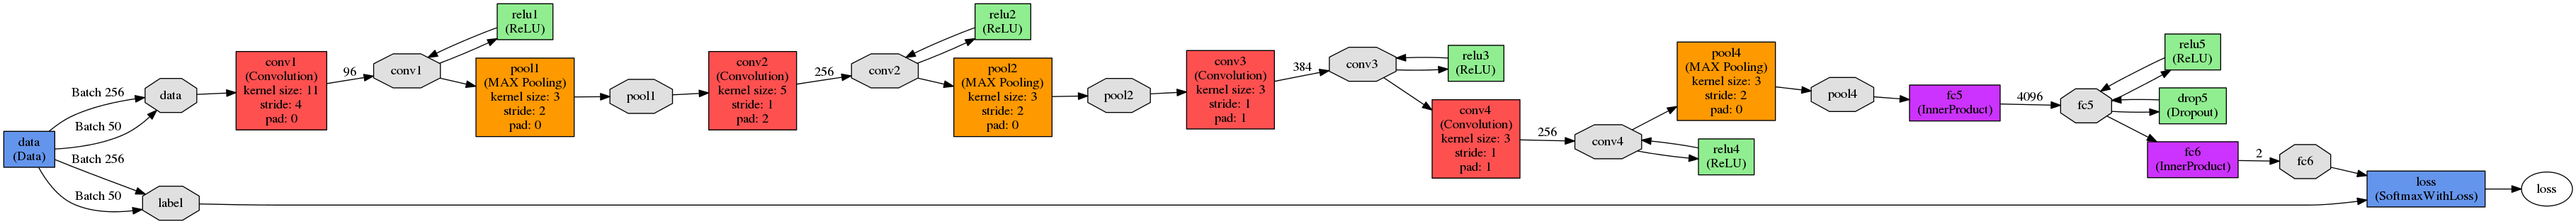
\includegraphics[page=1,width=0.95\textwidth]{net12.png}
		\caption{\label{fig:net12}{The single network architecture used as a baseline.}}
	\end{figure}
	
	The logic behind the architecture of the split networks results clearly from the parallel we can draw between the ADMM optimization algorithm and the networks architecture. Let us look at that more closely.
	
	In ADMM, we are trying to minimize an overall cost function, which in the case of a single, and hence also double, network corresponds to the classification accuracy of the image recognition task. The dual parameters that we use to optimize the augmented Lagrangian cost have to be then linked to the separated networks, let's call them \textbf{network 1} and \textbf{network 2} (later also called net1 and net2 for simplicity). Indeed, if we denote the output activations of a specific layer in network 1 as \textbf{x} and the activations of another layer in network 2 as \textbf{y}, then minimizing the squared norm $||x-y||$ is going to bring the two separate networks closer together. This is of course provided that the two designated layers exhibit topological similarity i.e. are architecturally the same and, what's most important, \textbf{share the same input}. This gives us a better idea of what the splitting should look like. We should try to separate the single network at a chosen point and let that point be a common input to:
	\begin{itemize}
		\item a remaining part of the agreed network 1 architecture.
		\item the first layer of the network 2 architecture.
	\end{itemize}
	
	Naturally, this is easier understood pictorially, and is hence shown in figure \ref{fig:dual-training}. The 3 and 3' layers share the same input (which is the output of layer 2) and produce outputs that should be agreeing with each other as much as possible, or as much as the squared norm can be minimized.
	
	\begin{figure}[!h]
		\centering
		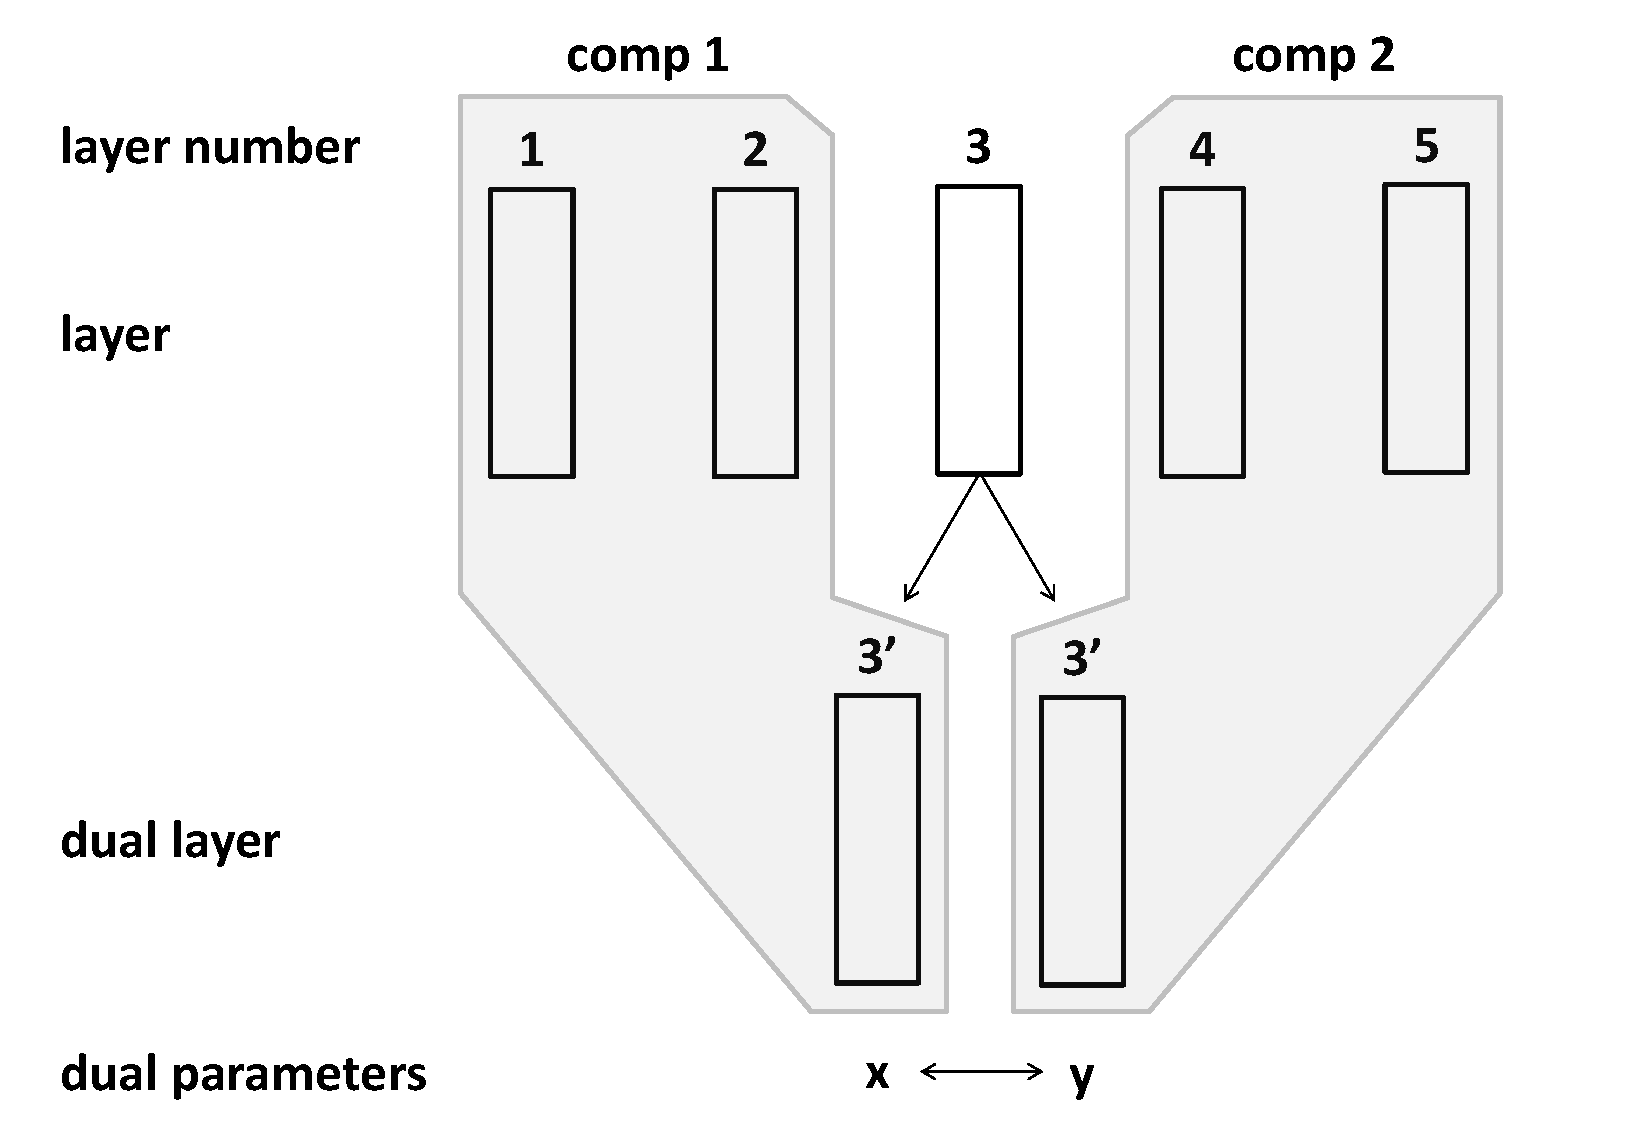
\includegraphics[page=1,width=0.60\textwidth]{dual-training.pdf}
		\caption{\label{fig:dual-training}{Breaking down the network between the machines}}
	\end{figure}
	
	The two are deemed as "dual" in the figure, because we are attempting to minimize the difference between them.
	
	Coming back to the equation \ref{ADMM_equation}, we can see why the two problems are similar. Noting that $\boldsymbol x$ and $\boldsymbol y$ above (the network parameters in the dual layers) can be treated identically to $x$ and $y$ in the equation, ADMM can help us minimise the difference between the two output vectors. This in turn will ensure that the distributed neural network training will be convergent to a common set of parameters for the network, albeit computed on separate machines.
	
	\section{Architecture}
	
	\subsection{Putting it all together}
	
	We can now collect all the pieces together and use the simplified figure \ref{fig:dual-training} to break down the actual network architecture used in the problem. As shown and mentioned before, the network architecture used is loosely based on CaffeNet and can be seen in figure \ref{fig:net12}. For clarity, it is also shown below in figure \ref{fig:net12pretty}.
	
	\begin{figure}[!h]
		\centering
		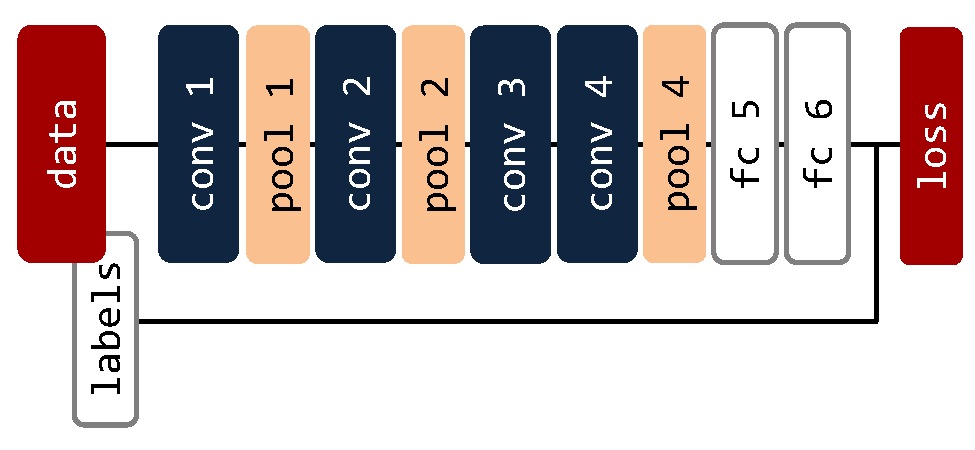
\includegraphics[page=1,width=0.6\textwidth]{net12.pdf}
		\caption{\label{fig:net12pretty}{The single network architecture used as a baseline.}}
	\end{figure}
	
	The network above is now distributed between two separate processing units as outlined above, and shown in the figure \ref{fig:net12separate} below.
	
	\begin{figure}[!h]
		\centering
		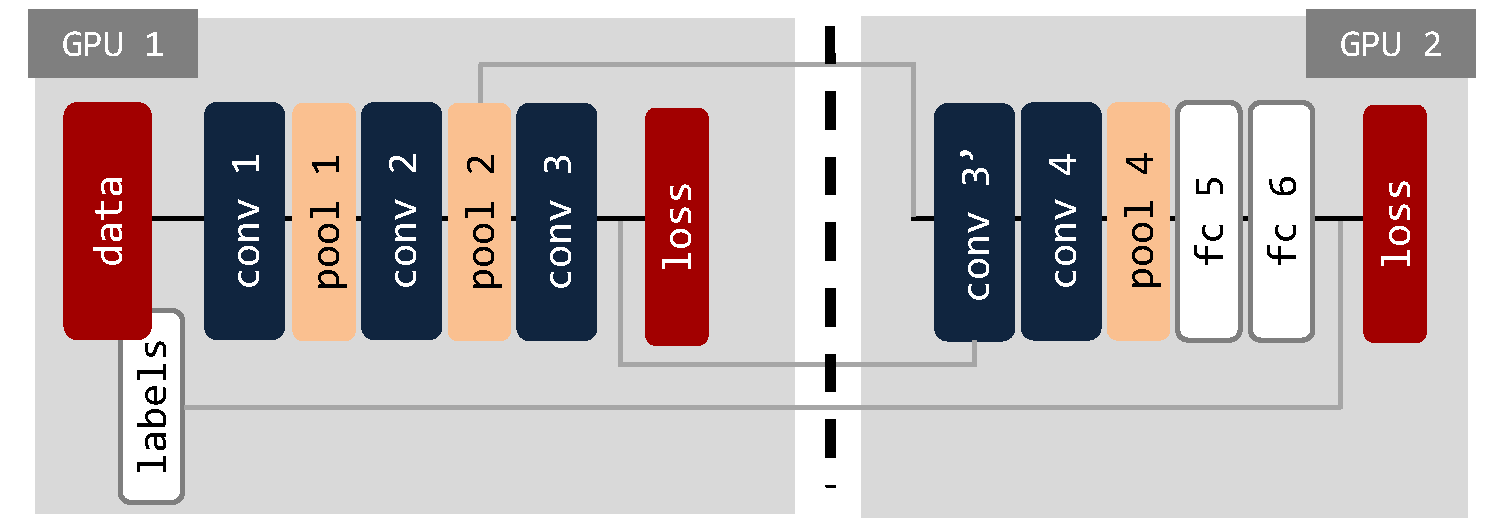
\includegraphics[page=1,width=0.9\textwidth]{net12separate.pdf}
		\caption{\label{fig:net12separate}{The dual networks imitating the single one.}}
	\end{figure}
	
	Putting the theory from before into practice, looking at the figures above we now note:
	\begin{itemize}
		\item The single network architecture consists of 4 convolutional layers, three of which are followed by a pooling layer. It is then split into two parts.
		\item network 1 (\textbf{net1}, on the left) consists of the original input data layer, the three convolutional data layers and a loss.
		\item network 2 (\textbf{net2}, on the right) has as its input the output of layer pool2. It consists of a dual conv3 (conv3') layer, followed by the original remainder of the network, including the loss.
		\item The loss computed in net1 is the difference between original conv3 and the one computed in the dual layer - conv3'.
		\item The loss computed in net2 is the difference between the computed image labels and the ground truth.
	\end{itemize}
	
	Assuming the correctness of ADMM, the above setup should let us run iterations on each of the nets sequentially, one after another. Ideally, to the outside world it will seem as if the computation was run on a single network. For completeness, the Caffe prints of the net1 and net2 architectures are included below.
	
	\begin{figure}[!h]
		\centering
		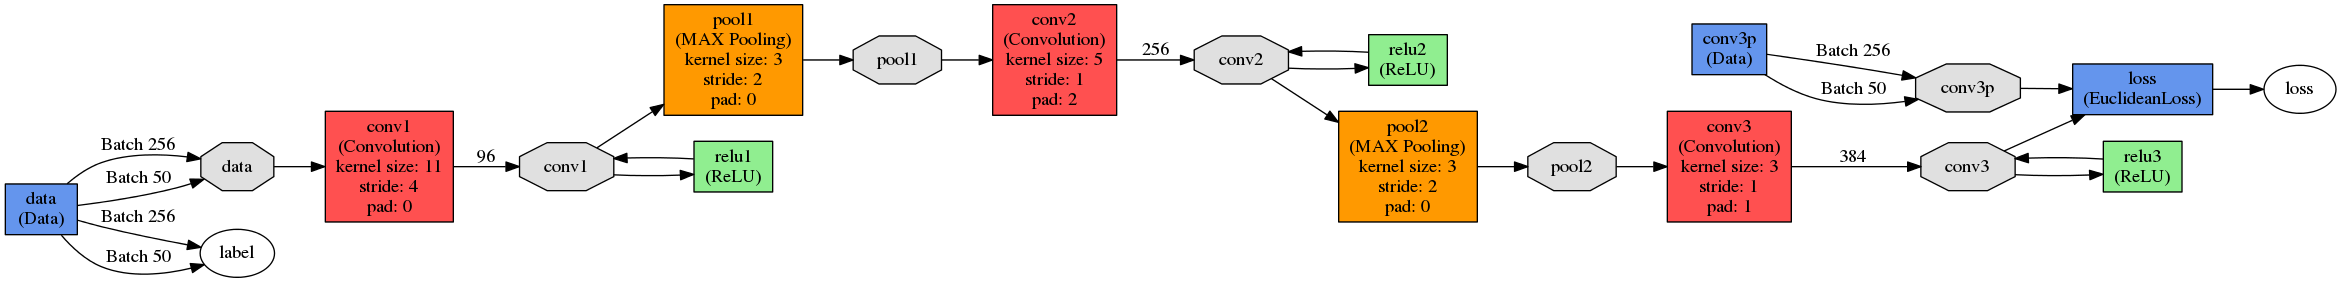
\includegraphics[page=1,width=0.9\textwidth]{net1.png}
		\caption{\label{fig:net1}{The Caffe net1 print.}}
	\end{figure}
	
	\begin{figure}[!h]
		\centering
		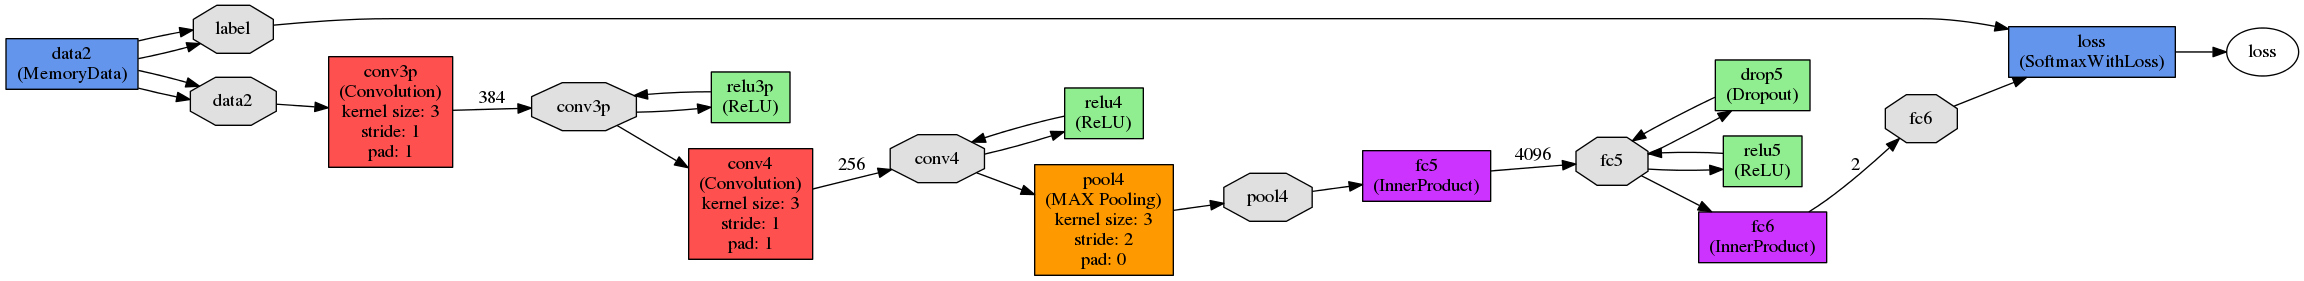
\includegraphics[page=1,width=0.9\textwidth]{net2.png}
		\caption{\label{fig:net1}{The Caffe net2 print.}}
	\end{figure}
	
	\subsection{Dataset}
	
	Before we delve further into the intricacies of the dual network architectures let us just quickly summarize the dataset used for the training.
	
	Initially, the training set consisted of 10,000 images of cats and dogs, 5,000 each, of various dimensions. The animals presented in the images were captured in different positions and settings. The images were scaled into 227x227 resolution before the training.
	
	Even though useful for getting started, the dataset proved to be too computationally heavy for sufficiently quick prototyping. That is why the cifar10 dataset was used instead. It consists of CHECK THIS --->>>>>>>> 50,000 training images and 10,000 test images representing objects of 10 different classes, with 32x32px resolution.
	
	\subsection{Deep learning frameworks}
	Recent years have seen a tremendous rate of development of the field of deep learning, and, not surprisingly, a surge in the number of deep learning frameworks. Today the choice is abundant, and the main competitors vary significantly when it comes to performance, implementation and usability. Due to the very technical, low-level nature of the project, significant consideration was given to the choice of an appropriate framework.
	
	The most significant frameworks nowadays include Caffe, theano, torch and tensorflow by Google. There is also a number of overlying interfaces and wrappers, such as Keras. The prototype was decided to be built in Caffe for several reasons:
	
	\begin{itemize}
		\item It has got a well-developed python interface and API.
		\item It is endorsed as not having a very steep learning curve.
		\item There is a big community support for it.
	\end{itemize}
	
	All of the above certainly come at a cost, though:
	
	\begin{itemize}
		\item As much as it is well supported, Caffe is not very well documented. It's hard to dig into the intricacies of its python API at times.
		\item Even the python interface requires the usage of prototxt files to define the model architecture and solver details. That reduces the clarity of the overall codebase.
	\end{itemize}
	
	With all of its pros and cons weighted up, Caffe was decided to be the right tool for prototyping, and hence it was used throughout the first stages of the project, It is absolutely possible and rather advisable to check the feasibility of the described solutions in a different framework.
	
	\subsection{Caffe tricks and quirks}
	
	Even with the architecture meticulously planned out and the objectives very clear, the implementation of the prototype turned out to be a very challenging tasks. Sadly, this was not due to the inconsistencies in the model laid out in the previous sections, but rather due to the erratic documentation of Caffe. The most challenging issues encountered during prototyping were:
	
	\begin{enumerate}
		\item \textbf{Running the forward and backward pass of net2 separately}. The default Caffe interface for carrying out one iteration of learning is "solver.net.step(1)" and it runs a forward and backward pass through the net as well as the weight update. As it turns out, this is surprisingly very difficult to do in steps using the predefined functions.
		\item \textbf{Updating the input of net2}. As mentioned earlier, the input to net2 is dynamic - it changes with every iteration, because the output of the pool2 layer changes. It is, again, surprisingly difficult to achieve the desired effect.
	\end{enumerate}
	
	Fortunately, extensive research of the Caffe websites and fora helped solve many of the above problems, notably (in the same order):
	
	\begin{enumerate}
		\item Caffe interface offers the "solver.net.forward()" and "solver.net.backward() functions which complete two of the three required iteration steps, with the other one being the weight update. Even though Caffe offers little automation for that, it can and was done manually, by investigating the "blob.diff" value for each of the parameter matrices (blobs in this case). The "diff" contains the gradient of a specific weight with respect to the overall loss function, and hence if multiplied by the negative learning rate it should return the needed weight update:
		\begin{equation}
		w^{t+1} = w^t + \Delta w = w^t - \mu \frac{\delta L}{\delta w}
		\end{equation}
		\item At first, the dynamic data layer update was done manually by just overwriting the contents of a randomly initialized layer.  It turned out to be a flawed approach because Caffe does not allow for a manual update of an operational data layer. Even though the values seem to be updated when queried, calling the forward pass function brings them back to the original values. Caffe does have several types of data layers, though, and one of them - MemoryData - turned out to be particularly useful for our application. The data layer is not initialized until the desired data is manully fed into it in the python code, which also allows for dynamic updates between iterations. This also preserves the updated data when forward and backward passes are called.
	\end{enumerate}
	
	A very similar technique to the one described above was used for communicating the layer conv3p (or conv3') data to net1. The communication was required because the loss of net1 is defined as the norm difference between the dual conv3 and conv3p layers. The data was hence simply copied from net2 and pasted manually into a MemoryData data layer in net1 before the loss computation.
	
	There are several ways to implement the \textbf{network communication}. Initial drafts of the framework revolved around using tcp sockets to send the appropriate data in an in-order, error-free manner. Fortunately, the architecture of the server cluster used for the training took advantage of a shared file system, which could be accessed from each of the distinct processing units. That is why the desired parameters were just saved as numpy ".npy" files and easily accessed by the other part of the algorithm at the appropriate stage.
	
	One more technical nuance we should mention is the synchronization between the networks. Similarly to the method above, the nets saved the details about their current computation stages in a shared file that could be probed if needed.
	
	\section{The algorithm}
	
	After introducing all the necessary theoretical, architectural and practical insights about the requirements of the project we are now able to design the algorithm used for the dual net training. As stated before, the algorithm is going to try to imitate the \textbf{alternating direction method of multipliers} algorithm. As the name suggests, we are then going to try to optimize the dual nets separately in an alternating manner - that means we will focus on minimizing the loss function of only one of them at any one time. This is achieved by the algorithm summarized in figure \ref{fig:algorithm}.
	
	\begin{figure}[!h]
		\centering
		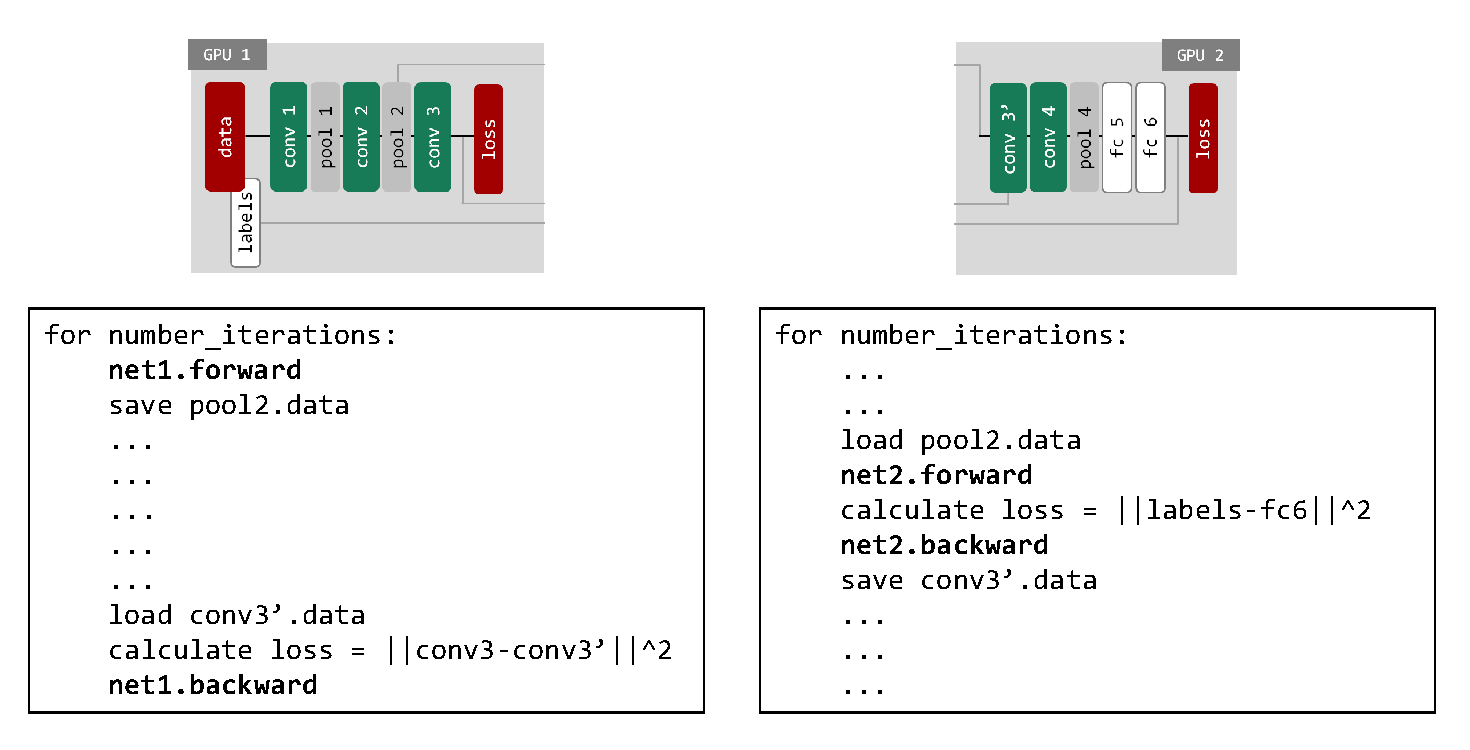
\includegraphics[page=1,width=0.9\textwidth]{algocode.pdf}
		\caption{\label{fig:algorithm}{The algorithm used for dual network training.}}
	\end{figure}
	
	The first step of the algorithm is the forward pass of network 1. This produces the initial layer activations and, importantly, the output of the pool2 layer. This is saved into a file and communicated to the rest of the program running on a separate GPU.
	
	For the second step we move to net2. It first retrieves the data communicated by net1 earlier and loads in onto its data layer. It then runs a complete training iteration including forward and backward pass followed by the parameters update. The backward pass minimizes the difference between the image labels computed during the forward pass and the ground truth. Net2 then saves the data computed for the dual conv3p layer.
	
	We now move back to net1. It first loads the conv3p layer data and computes the norm difference between the dual conv3 and conv3p layers. This is net1's cost function, and hence during the backward propagation the solver calculates parameter gradients that lead to minimization of the norm. After the backprop is done, we are ready to carry out the final pass through the network and use the computed gradients to update the weights appropriately.
	
	After the weight update one complete iteration of the whole setup is done. We have hopefully:
	
	\begin{enumerate}
		\item Minimized the difference between the dual layers.
		\item Minimized the overall loss, which is akin to training the single network (and should make the two indistinguishable from the outside world).
	\end{enumerate}
	
	We can then repeat the above procedure for a few thousand iterations or until some convergence criterion is met.
	
	\section{Testing}
	
	The meticulously planned setup above then required a thorough heuristic validation. The hardware used to test the algorithms was a single Nvidia GeForce GTX Titan Graphical Processing Unit for each network, hence two of them in total, placed on two distinct servers within a cluster.
	
	Deep neural networks, particularly as implemented by one of the modern frameworks, often involve a complex programmatic setup. In our case, an additional level of complexity is introduced by the fact that the network topology is divided between several computational units. All of this results in a very high sensitivity of the model to the input parameters, and further emphasises the need for meticulous planning and thorough understanding of the framework at hand. Naturally, both come easier with sufficient practice and a fair bit of heuristic trialling which became a significant part of the project. The next few sections will present the variability of the model with respect to some of the parameters and will then progress to describe the testing of the dual setup with various parameter combinations.
	
	\section{Technical difficulties}
	
	Naturally, many problems were encounted before the network started exhibiting the desired behaviour. Most of them were linked to the issues described in an earlier section, namely:
	
	\begin{itemize}
		\item Net2 was not converging because the dynamic data layer update was not behaving as expected.
		\item Net1 was not converging because the parameters were not appropriately updated based on the computed gradients.
	\end{itemize}
	
	The solutions to these are mentioned in the previous sections as well.
	
	Once initial performance metrics started looking positive, i.e. both net1 and net2 losses decreased as the training proceeded, some baseline results and conclusions could have been drawn.
	
	\subsection{Two objectives}
	
	Let us shortly remind ourselves about the dual setup topology used (fig. \ref{fig:net12separate}). We break down our big network in such a way that one of the layers is duplicated in both of the individual, smaller nets. The two nets are then trying to:
	\begin{enumerate}
		\item Converge in order for the two "dual layers" to become nearly identical.
		\item Converge in order to match the ground truth of the classification predictions.
	\end{enumerate}

	These two objectives are manifested through the two losses, one for each network. The loss for network 1 tries to minimize the difference between the dual layers, whereas the one for network 2 aims to classify the images correctly.
	
	Losses that are optimized by the Stochastic Gradient Descent algorithm are in Caffe calculate and represented by layers. A lot of them are available out-of-the-box and even in the default version of Caffe provide reasonable space for fine-tuning the network. In some cases, though, the default layers are not sufficient to achieve the necessary metrics, which is solved by implementing custom layers in C++ or in the Python interface.
		
	There is little variability in choosing the correct architectural setup to achieve the second convergence objective above. The loss is based on the similarity between the image labels produced by the trained network, and the ground truth. Both are represented as a vector with values corresponding to the probabilities of image classification into each of the classes. The loss is then calculated according to the formula for the cross-entropy classification loss:
	\begin{equation}
		E = \frac{-1}{N} \sum_{n=1}^{N} log(\hat{p}_{n,l_n})
	\end{equation}
	
	where $\hat{p}_n$ are the probability classes and $l_n$ are the true labels.
	
	\subsection{Net 1 loss}
	
	Unfortunately, the choice of the loss function is not as trivial when it comes to the first convergence objective. It quickly turned out that the default loss layers offered in Caffe are not sufficiently customizable to cater for our needs, hence a custom setup was built instead. Before we delve into the details, though, let's start off with a more fundamental analysis of what we want to achieve.
	
	How do we define identical? The convolutional layers we are dealing with are huge, four-dimensional matrices as opposed to simple two-dimensional vectors, hence a more involved similarity metric is required for the comparison. Fortunately, the laws and metrics in linear algebra easily generalize to higher dimensions. Hence, to compare the convolutional dual layers we can use a simple Euclidean loss, as defined by:
	
	\begin{equation}
		E=\frac{1}{2N} \sum_{n=1}^{N} ||\hat{y}_n-y_n||^2_2
	\end{equation}
	
	Fortunately, this is the functionality offered out-of-the box by Caffe's default Euclidean Loss Layer. Ideally, we would then expect the loss layer to minimize the difference between the dual convolutional layers, and let the net2 loss force convergence with respect to the true image labels. After giving the approach a go, however, some very interesting insights have been discovered.
		
	\subsection{Default Euclidean Loss Layer in practice}
	
	Both of the training losses computed throughout training seemed to be very volatile. Before we jump into the exact analysis of the problem, though, let's revisit the idea of the stochastic gradient descent. The gradient of the loss function computed by SGD is based on a random sample of the training set, which in our case is 256 images out of 10,000. This is clearly not representative of the whole population on its own, however over many iterations it should converge to a representative average. This is precisely what happens in our case. The losses computed after each iteration seem volatile, however over many iterations they do exhibit convergence. The stochastic batches we use for updating the loss are big enough for global minimization over a long time, but too small to produce a consistent trend at every iteration. This should not be a concern, though, as long as the general trend is visible.
	
	The point above concerns both net1 and net2, however it is clearly more pronounced in the latter, hence more consideration is given into the possible explanations. Due to the nature of the algorithm, we are building up gradually more volatile calculations, hence the loss of net2 can be expected to vary more. In particular, it should be noted that the input of net2 is not constant, but varying with every iteration adding to the overall volatility.
	
	After all, both of the nets seemed to be converging, which can be clearly seen in figure \ref{fig:default_losses}. After more tests were carried out, however, it seemed that the convergence of net2's loss is rather dubious. The results weren't always repeatable, and even the "successful" cases have confirmed that local variance in the loss computations was bigger than the overall convergence trend.
	
	\begin{figure}[!h]
		\centering
		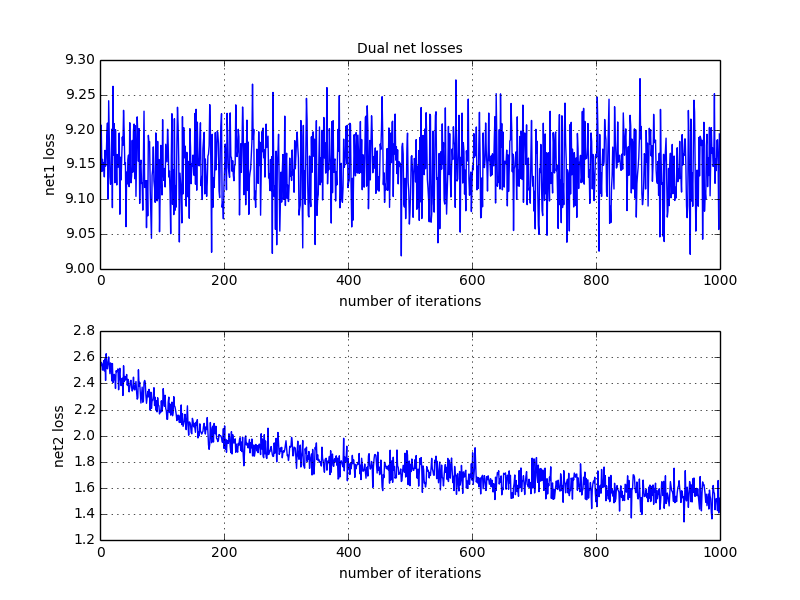
\includegraphics[page=1,width=0.9\textwidth]{losses.png}
		\caption{\label{fig:default_losses}{The training losses for the prototype framework.}}
	\end{figure}
	
	The pessimistic conclusions were further confirmed by running a classification task using a trained model. Out of a 1000 test samples, only about 100 were classified correctly. 1 in 10. This was suspiciously close to the number of image classes, which suggested that our method is virtually equivalent to random guessing.
	
	After setting up more probing mechanisms within the code an interesting pattern was spotted. As the training progressed, the convolutional layers produced consecutively smaller data i.e. the norm of the output matrices decreased with every iteration. The reason for this is apparent when we try to understand the objective of the loss layer - \textbf{to minimize the difference between the two convolutional layers}. What does that mean? That we are either going to:
	\begin{enumerate}
		\item Force the values of the convolutional layers' outputs close together.
		\item Make the outputs small enough that no matter what the relative difference between them is, the absolute one is going to be tiny!
	\end{enumerate} 
	
	The second point explains the exponentially decreasing net1 loss in figure \ref{fig:default_losses}. At the end of the training, all that the network produces is matrices of zeroes, which are indeed close to each other, but do not satisfy our second training objective - to get closer to the correct classification.
	
	Some mechanism had to be put in place which would inhibit the layer from optimizing its objective by simply making all of the values tiny. That mechanism is normalization - we do not want the absolute value of the conv layers' difference to be small - we just want it to decrease relative to what the current norm size of the layers is.
	
	\subsection{Custom Euclidean Loss Layer}
	
	None of the built-in Caffe mechanism allowed for introducing a normalization term to the euclidean loss. Fortunately, Caffe does allow for custom layer creation which made it possible to define a \textbf{Euclidean Loss Layer with Normalization}.
	
	Conveniently, the examples online (\cite{caffe2016loss}) provided a custom python implementation of the Euclidean Loss Layer analysed before. It was decided to first contrast the performance of the layer found online in order to build the normalized loss layer on a proven baseline. The below code listing shows the parameter update step during forward propagation of the network.\\
	
	\begin{lstlisting}
	def forward(self, bottom, top):
	    self.diff[...] = bottom[0].data - bottom[1].data
	    top[0].data[...] = np.sqrt(np.sum(self.diff**2)) / bottom[0].num / 2.
	\end{lstlisting}
	
	The results were again very interesting. The second convergence objective was clearly satisfied - the classification loss was decreasing with every iteration, which brought us a step closer to competing with a singular topology. What was worrying, though, that the first convergence objective wasn't satisfied at all - no decreasing trend could have been identified in the training loss of the first part of the network. This is clearly seen in the figure \ref{fig:incorrect_custom_training} below.
	
	\begin{figure}[!h]
		\centering
		\includegraphics[page=1,width=0.9\textwidth]{incorrect_custom_training.png}
		\caption{\label{fig:incorrect_custom_training}{The losses for both of the networks during the first iteration of training using a custom Euclidean loss layer.}}
	\end{figure}

	To trace down the reason for net1's flat learning curve the gradients of the individual net parameters with respect to the overall loss were probed. Not surprisingly, it turned out that they were all zero, leading to virtually no learning. The reason for that turned out not to be architectural, but rather technical - the custom python layers in Caffe have to be identified in the training .prototxt file by annotating them with "loss\_weight: 1". Otherwise no backpropagation is ran any of the layers backing the final one. After fixing the technical inconsistency, backpropagation on all the appropriate layers was run and the gradients were indeed calculated correctly.
	
	What is interesting, though, is that the above setup, alas largely incorrect, achieved surprisingly high classification results. On a testing sample of a 1,000 images, it managed to correctly identify the labels of 52.53\% of them. This can be contrasted to the classification accuracy of 63.75\% of the single network setup.
	
	The impressive conclusion from the above is that since the bottom part of the dual network was virtually useless (its loss was constant throughout the training), all learning has occured in the latter part i.e. only using one convolutional layer. This is truly remarkable, given how close the classification accuracy was to the fully-leveraged single-net architecture.
	
	Even though the architecture was imperfect, it was decided to test the network with big data batches and compare their size to the maximum that can be fitted on the singular network topology.
	
	\subsection{Big batch}
	
	To run the tests, the batch size was increased to twice its previous size every time until it filled up the memory of the GPU completely. It turned out that:
	\begin{itemize}
		\item The biggest batch size that can be fitted on the single net topology is 2608 samples.
		\item The biggest batch size that can be fitted on the dual net topology is 4095 samples.
	\end{itemize}
	
	These results are outstanding - by breaking down the network between two units, we were able to increase the amount of data that can be processed on them together by a factor of two.
	
	The significance of these results can be explained in terms of several deep learning facts:
	\begin{enumerate}
		\item A bigger mini-batch helps to streamline the calculations executed with every training iteration. In simple terms, comparable convergence of a network using only one image in a batch will take N times longer than training of an identical network with a mini-batch size of N. \\ In theory, the same number of operations is going to be performed. The computational cost of multiplying big matrices is however smaller than the cost of doing those operations during separate iterations. Additionally, less time is spent on propagating the results throughout the network i.e. fewer forward- and backpropagations are concluded before convergence.
		\item Regardless of the batch size, one certain conclusion is that we can fit a lot more data on the network. An alternative to increasing the batch size is increasing the number of convolutional layers. This can prospectively lead to higher classification results, because exponentially more complex functions can be learnt with incrementally increasing network sizes.
	\end{enumerate}

	\begin{figure}[!h]
		\centering
		\includegraphics[page=1,width=0.9\textwidth]{big_batch.png}
		\caption{\label{fig:big_batch}{Training curves of the single and dual network setup using maximum batch sizes (2608 samples in single and 4096 samples in dual).}}
	\end{figure}

	The figure \ref{fig:big_batch} shows the training curves for both of the network architectures using maximal mini-batch sizes. The learning curves are clearly smooth at times but also exhibit some spiking behaviour. This can be easily explained.
	
	The smoothness comes from low variance of the gradient calculations. The bigger the mini-batch, the more representative it is of the whole population, and hence it can guarantee very stable gradient descent.
	
	On the other hand, the stochasticity of the gradient descent is somewhat lost as the batch increases. The spikes occur because the loss function is getting trapped in local minima of the loss functions that would normally be quickly escaped fromt thanks to probabilistic choice of the samples forming the dataset.
	
	\subsection{Normalization term }
	
	It became very clear that the need for normalization of the training loss in net1 is compelling. The first approach to the loss normalization involved dividing it by the sum of the 2-norms of both of the convolutional layers. This can be neatly represented as:
	
	THIS IS PROBABLY WRONG
	
	\begin{equation}
		E=\frac{1}{2N} \sum_{n=1}^{N} \frac{||\hat{y}_n-y_n||^2_2}{||\hat{y}||^2_2+||y||^2_2} 
	\end{equation}
	
	It was hoped that the normalization term will make the loss values consistent, and then attempt to indeed minimize the difference between them instead of just bringing the absolute parameter values close to zero. As shown in figure \ref{fig:exploding_values}, this first attempt at normalization did not result in a significant improvement in performance. The loss values were indeed bounded to comparable values (the loss decrease was not exponential as before), but dropped to zero very quickly. After that, the outputs of the layers quickly overflowed. \\
	
	\begin{figure}[!h]
		\centering
		\includegraphics[page=1,width=0.9\textwidth]{exploding_values.png}
		\caption{\label{fig:exploding_values}{It turned out that introducing the normalization term helped bound the loss values a little, but still led to very unstable behaviour afterwards}}
	\end{figure}
	
	Figure \ref{fig:plus_equals} shows yet another variation on the testing parameters in order to find the error in the network architecture setup. The sign of the parameter update in each of the layers was flipped, as shown in the line 5 below: \\
	
	\begin{lstlisting}
	# backprop and weight update
	solver.net.backward()
	for layer in solver.net.layers:
	    for blob in layer.blobs:
 	        blob.data[...] += learningRate*blob.diff
	\end{lstlisting}
	
	Not surprisingly, it resulted in network 1 loss increasing, which at least confirmed that the parameter update was in the right direction. What was surprising, though, was that the image classification loss did exhibit a decrease, before it exploded into highly overflown numbers.
	
	\begin{figure}[!h]
		\centering
 		\includegraphics[page=1,width=0.9\textwidth]{plus_equals.png}
		\caption{\label{fig:plus_equals}{In the pursuit of the errors, several different network setups were tested. This one involved changing the sign of the gradient addition.}}
	\end{figure}
	
	\subsection{Learning rate}
	
	In the pursuit of a solution to the dual convergence problem many attempts were made at adjusting the model parameters in order to achieve more promising results. One to which the convergence seemed particularly sensitive was, not surprisingly, the learning rate. While researching the possible explanations for devastatingly rapid convergence or increasing loss function, many specialist forums suggested adjusting the learning rate as one of the main factors affecting the training. Sadly, in most of the cases the learning rate affected just that - the rate of learning, the speed at which our network is approaching the value it is converging to. Apart from a couple of extreme cases (not worth mentioning), varying the learning rate simply stretched or shrinked the learning curve across the iterations appropriately. This can be very vividly seen on figure \ref{fig:learning_rate_variation}, where the two networks were trained using the same parameters and under identical circumstances, save the learning rate which differed by a factor of a 100 between the two.
	
	\begin{figure}[!h]
		\centering
		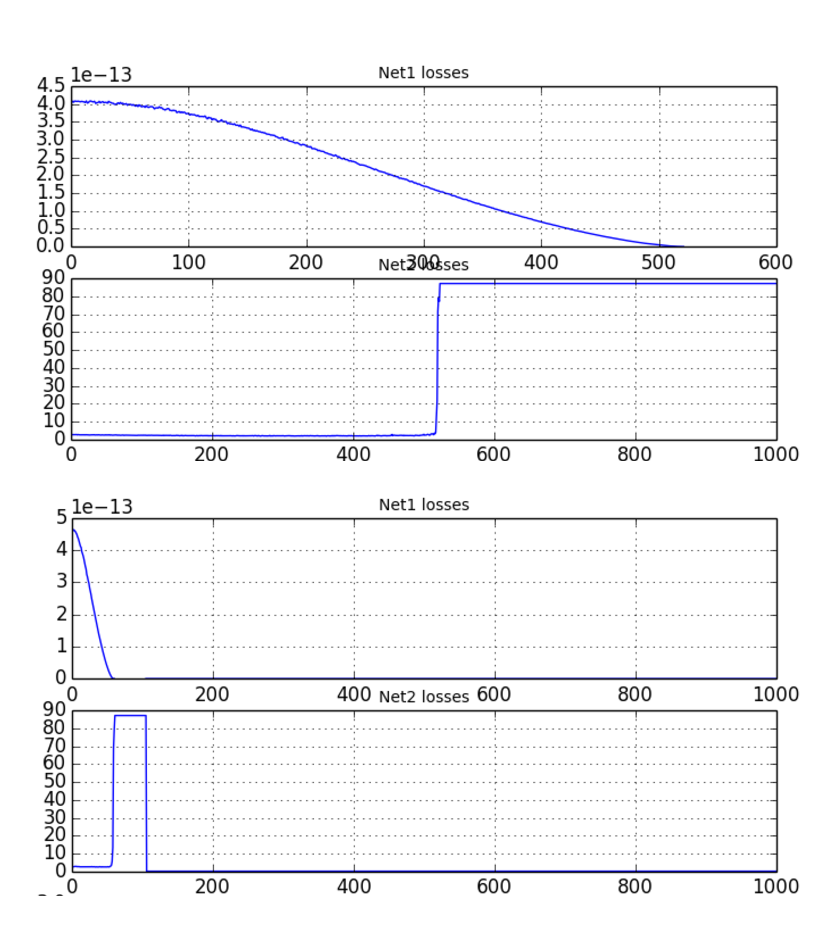
\includegraphics[page=1,width=0.7\textwidth]{learning_rate_variation.pdf}
		\caption{\label{fig:learning_rate_variation}{It is clear that in most of the cases varying the learning rate changed just that - the rate at which we are approaching convergence. The above nets were trained using the same parameters and under identical circumstances, save the learning rate which differed by a factor of a 100 between the two.}}
	\end{figure}
	
	
	
	
	
	\newpage
	\clearpage
	\subsection{things to do in this report}
	\begin{enumerate}
		\item label listings]
		\item download some python syntax coloring
		\item swap the figures to something that is not crap
		\item figure out the right formulae for normalization
		\item up to normalization part, everything should be okay. Later it's wild
	\end{enumerate}
	
	
	\newpage
	
	\clearpage
	
	\newpage
	\pagestyle{plain}
	\bibliography{bib}
	\bibliographystyle{abbrv}
	
	
\end{document}

